\documentclass[11pt,hyperref]{ctexart}
\usepackage{lmodern}
\usepackage{amssymb,amsmath}
\usepackage{ifxetex,ifluatex}
\usepackage{fixltx2e} % provides \textsubscript
\ifnum 0\ifxetex 1\fi\ifluatex 1\fi=0 % if pdftex
  \usepackage[T1]{fontenc}
  \usepackage[utf8]{inputenc}
\else % if luatex or xelatex
  \ifxetex
    \usepackage{xltxtra,xunicode}
  \else
    \usepackage{fontspec}
  \fi
  \defaultfontfeatures{Mapping=tex-text,Scale=MatchLowercase}
  \newcommand{\euro}{€}
\fi
% use upquote if available, for straight quotes in verbatim environments
\IfFileExists{upquote.sty}{\usepackage{upquote}}{}
% use microtype if available
\IfFileExists{microtype.sty}{%
\usepackage{microtype}
\UseMicrotypeSet[protrusion]{basicmath} % disable protrusion for tt fonts
}{}
\usepackage[margin=1.5in]{geometry}
\ifxetex
  \usepackage[setpagesize=false, % page size defined by xetex
              unicode=false, % unicode breaks when used with xetex
              xetex]{hyperref}
\else
  \usepackage[unicode=true]{hyperref}
\fi
\usepackage[usenames,dvipsnames]{color}
\hypersetup{breaklinks=true,
            bookmarks=true,
            pdfauthor={胡弘宇},
            pdftitle={R 入门指引 (The path of learning R)},
            colorlinks=true,
            citecolor=blue,
            urlcolor=blue,
            linkcolor=magenta,
            pdfborder={0 0 0}}
\urlstyle{same}  % don't use monospace font for urls
\usepackage{graphicx,grffile}
\makeatletter
\def\maxwidth{\ifdim\Gin@nat@width>\linewidth\linewidth\else\Gin@nat@width\fi}
\def\maxheight{\ifdim\Gin@nat@height>\textheight\textheight\else\Gin@nat@height\fi}
\makeatother
% Scale images if necessary, so that they will not overflow the page
% margins by default, and it is still possible to overwrite the defaults
% using explicit options in \includegraphics[width, height, ...]{}
\setkeys{Gin}{width=\maxwidth,height=\maxheight,keepaspectratio}
\usepackage[normalem]{ulem}
% avoid problems with \sout in headers with hyperref:
\pdfstringdefDisableCommands{\renewcommand{\sout}{}}
\setlength{\emergencystretch}{3em}  % prevent overfull lines
\providecommand{\tightlist}{%
  \setlength{\itemsep}{0pt}\setlength{\parskip}{0pt}}
\setcounter{secnumdepth}{0}

\title{\(R\) 入门指引 (The path of learning R)\\\vspace{0.5em}{\large \url{https://github.com/jun3970/R-Intro}}}
\author{胡弘宇}
\date{05 June 2020}


\usepackage{paralist} \let\itemize\compactitem \let\enumerate\compactenum

% Redefines (sub)paragraphs to behave more like sections
\ifx\paragraph\undefined\else
\let\oldparagraph\paragraph
\renewcommand{\paragraph}[1]{\oldparagraph{#1}\mbox{}}
\fi
\ifx\subparagraph\undefined\else
\let\oldsubparagraph\subparagraph
\renewcommand{\subparagraph}[1]{\oldsubparagraph{#1}\mbox{}}
\fi

\begin{document}
\maketitle

\begin{quote}
R is a programming language and free software environment for
statistical computing and graphics supported by the R Foundation for
Statistical Computing.\\
--- The Comprehensive R Archive Network - R FAQ - What is R?
\end{quote}

\hypertarget{ux524dux8a00}{%
\subsection{前言}\label{ux524dux8a00}}

又是一年毕业季,导师(暨南大学经济学院谢子雄教授)提议,
让我为师门即将入学的新生撰写一份入门 R 语言的路径指引。\footnote{我到底该学
  R 还是 Python? 首先看导师给的项目(要求)和个人规划;
  其次二者并不冲突,对于非计算机专业的同学来讲,无论熟练掌握哪一门都是极好的。
  具体来说,R 的战场只有两个:统计计算和数据可视化。 而 Python
  的应用领域有: web
  开发、服务器运维、自动化测试、人工智能(机器学习)、网络爬虫。
  可以看出 Python
  并不是为了某一类业务岗而专门设计的程序语言(``胶水语言''),
  由于其本身并不专精,故大家多是将其作为次语言使用
  (其在国内声名这么火爆,和培训机构的狂轰乱炸,割大学生韭菜有很大关系)。}
得谢老师信任,诚惶诚恐,我尽力为之。
需要强调的是,本文基于个人视角与学习经验写就,固有弊病。
粗浅看法与建议,读者请审慎参考。

\begin{figure}
\centering

\includegraphics{images/R-logo.png}
\caption{R logo}
\end{figure}

\href{https://www.r-project.org/}{\(R\)}
是一门开源的专业统计计算语言,脱胎于贝尔实验室的 \(S\) 语言。\footnote{R
  的語法是來自 Scheme。Scheme 是一种函数式编程语言,遵循极简主义哲学,
  以一个小型语言核心作为标准,加上各种强力语言工具(语法糖)来扩展语言本身。
  著名计算机科学入门教材《计算机程序的构造和解释》(SICP)利用 Scheme
  來解释程序设计。
  \href{https://www.wikiwand.com/zh/Scheme}{Wikipedia:Scheme}}
依托于其灵活强大的统计计算与数据绘图功能,
加之语言较易理解(核心开发团队中专业统计人员占大多数),拓展包(package)丰富,
R
成为当前学术界(尤其是统计、生物、经济等学科)最青睐的量化工具之一。\footnote{\href{https://cran.r-project.org/web/packages/available_packages_by_date.html}{Table
  of available packages, sorted by date of publication}. There are two
  major types of programming languages: low-level languages and
  high-level languages. Low-level languages are referred to as `low'
  because they are very close to how different hardware elements of a
  computer actually communicate with each other. A high-level language
  is a programming language that uses English and mathematical symbols,
  like +, -, \% and many others, in its instructions. When using the
  term `programming languages,' most people are actually referring to
  high-level languages, like as R.
  \url{https://study.com/academy/lesson/machine-code-and-high-level-languages-using-interpreters-and-compilers.html}}
2009 年 1 月 6 日被纽约时报科技版专文报导
\href{https://www.nytimes.com/2009/01/07/technology/business-computing/07program.html}{Data
Analysts Captivated by R's Power}. 我们可以在
\href{https://cran.r-project.org/mirrors.html}{CRAN} 免费获取 R
的安装文件与官方文档。\footnote{CRAN, 全称 Comprehensive R Archive
  Network. 是 R 官方组织维护的 R 资料讯息聚集地。
  网页样式虽停留在上一个世纪,但该有的干货一点儿也不少!
  为提高取得数据的网速,我们往往需要选择一个距离较近的镜像,大陆地区推荐清华或北外的镜像。
  此外,通过 R 的官方主页 \url{https://www.r-project.org/}
  我们可以实时了解 R 的最新动态。 对学习者而言,最宝藏的当属左侧
  Documentation 栏目下的内容。} RStudio 公司为我们提供了一款非常棒的开源
R 语言集成开发环境(IDE)---RStudio。\footnote{RStudio::conf
  是北美地区的数据科学盛会,会议报告人大体为热门 R
  包开发者,数据科学从业者,以及具有使用 R
  丰富经验的技术爱好者。会议报告的材料与现场视频(2017 年至今)被收录在
  RStudio 官网下的
  \href{https://rstudio.com/resources/webinars/}{Webinars \& Viedos}
  栏目(需要外网环境才能快速方便地访问,国内用户可到其维护的
  \href{https://github.com/jun3970}{Github} 仓库(repository)
  \href{https://github.com/rstudio/rstudio-conf}{rstudio-conf}
  获取会议幻灯片), 善加利用这些材料,成为 R 前沿用户不在话下。
  统计之都上有一篇 RStudio 公司创始人 J.J. Allaire
  接受记者专访的\href{https://cosx.org/2016/11/interview-j-j-allaire/}{翻译稿},感兴趣的可前往阅读。}

一本好的教材能极大地降低读者的学习成本。 而网络上关于 R
的学习资料琳琅满目,新手难免陷入选择的困惑。
本文以推荐优秀教材为主体内容(有一定 R
基础的读者直接点击文内链接到相应页面阅读即可),
说明性文字和补充材料读者可选择性撷取。
本文推荐书籍的标准是,书籍作者本身就是开发人员或统计学家(内容质量有所保证),
开源为先(利于获取,作者会随时更新)。\footnote{这几本书籍的学习理解难度大体上保持了由易到难的顺序。
  需要强调的是,我比较在意书籍内容的特征性与代表性,因为互补性学习能让我们将
  R 掌握地更加牢固精深。 (除了 \emph{Advanced R} 与 \emph{Applied
  Econometrics with R},其他书籍本人皆从头到尾地读过)。 Github
  是世界上最大的代码存放网站和开源社区, 绝大多数的 R 包源码都托管于
  Github, 当 \emph{CRAN} 上某包未及时更新(稳定版),我们可通过 devtools
  包中的 \texttt{install\_github()} 函数 直接从 Github
  仓库安装最新开发版(evelopment version)。}

若读者手头没有本地的数据项目需要处理,
建议读者在阅读学习过程中\sout{有选择地}\textbf{敲键盘复盘书中例子}(尤其是理解起来吃力的部分)。
若读者在学习过程中能做到时常尝试换一种写法,实现相同的程序目的,那么读者很快就能入门
R。 因为 R
语言不难于理解,单难于理解其语法逻辑(向量化)后的持续性使用,典型情境就是学了就忘
(手头有感兴趣的数据项目,还有人 push 你思考,则此问题迎刃而解)。
此外,微小的写法差异累积起来就是自己的 R 代码风格。

\begin{center}\rule{0.5\linewidth}{0.5pt}\end{center}

\hypertarget{ux5165ux95e8ux91cfux5316ux5206ux6790ux6570ux636eux79d1ux5b66}{%
\subsection{入门量化分析(数据科学)}\label{ux5165ux95e8ux91cfux5316ux5206ux6790ux6570ux636eux79d1ux5b66}}

\hypertarget{a.-the-r-for-data-science-import-tidy-transform-visualize-and-model-data-by-garrett-grolemund-hadley-wickham---oreilly-media}{%
\subsubsection{\texorpdfstring{A. \href{https://r4ds.had.co.nz/}{The R
for data science: Import, Tidy, Transform, Visualize, and Model Data} by
Garrett Grolemund, Hadley Wickham - O'Reilly
Media}{A. The R for data science: Import, Tidy, Transform, Visualize, and Model Data by Garrett Grolemund, Hadley Wickham - O'Reilly Media}}\label{a.-the-r-for-data-science-import-tidy-transform-visualize-and-model-data-by-garrett-grolemund-hadley-wickham---oreilly-media}}

\textbf{本书不适合具有其它统计语言编程经验(SAS, Stata 等),想直接上手
R 做统计计算的应用统计者。} 本书适合两类读者:

\begin{enumerate}
\def\labelenumi{\arabic{enumi}.}
\item
  对数据的认知与实践大体为做描述性统计,当下想入门 R,
  在论文中做一些稍微复杂点的量化分析工作。典型如社会科学专业的本科生和低年级研究生
\item
  了解 R 基本语句的大致用法,对 R 中当前热火朝天的 tidyverse
  感兴趣的数据科学爱好者
\end{enumerate}

\begin{quote}
The tidyverse is an opinionated collection of R packages designed for
data science. All packages share an underlying design philosophy,
grammar, and data structures.\\
--- Hadley Wickham \footnote{此处必须跪舔一下 Hadley Wickham
  大佬,Hadley 供职于开源软件公司 RStudio,在 2019
  年其凭借自身在数据科学领域的卓出贡献获得统计学
  ``诺贝尔''奖---考普斯总统奖 (COPSS Presidents' Award)。获奖词为:
  Wickham was awarded the international COPSS Presidents' Award in 2019
  for ``influential work in statistical computing, visualisation,
  graphics, and data analysis'' including ``making statistical thinking
  and computing accessible to a large audience''.}
\end{quote}

\hypertarget{ux4ee5ux672cux4e66ux5165ux95e8-r-ux8bedux8a00ux7684ux4f18ux52bf}{%
\paragraph{以本书入门 R
语言的优势}\label{ux4ee5ux672cux4e66ux5165ux95e8-r-ux8bedux8a00ux7684ux4f18ux52bf}}

\begin{enumerate}
\def\labelenumi{\arabic{enumi}.}
\tightlist
\item
  本书叙述逻辑框架是数据分析的工作流程。
  阅读本书,能使读者对寻常数据项目的内容与流程有一个系统性的认知。
\end{enumerate}

\begin{figure}
\centering
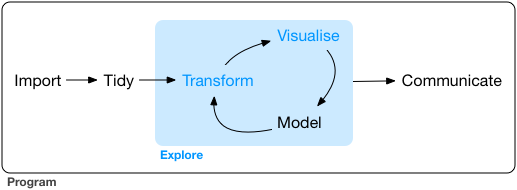
\includegraphics{images/data-science-explore.png}
\caption{数据分析工作流程}
\end{figure}

\begin{enumerate}
\def\labelenumi{\arabic{enumi}.}
\setcounter{enumi}{1}
\tightlist
\item
  书中对 \href{https://www.tidyverse.org/}{tidyverse}
  (极乐净土)做了系统且全面的介绍。 tidyverse
  系列包是一套以数据项目为内容对象的工具包。 其一定程度上重新包装了 R
  基础语句(尤其是管道符的加入),
  使得未有编程经验的新手能跳过细碎的语法细节,进入以函数为核心的数据操纵环节。
\end{enumerate}

\begin{figure}
\centering
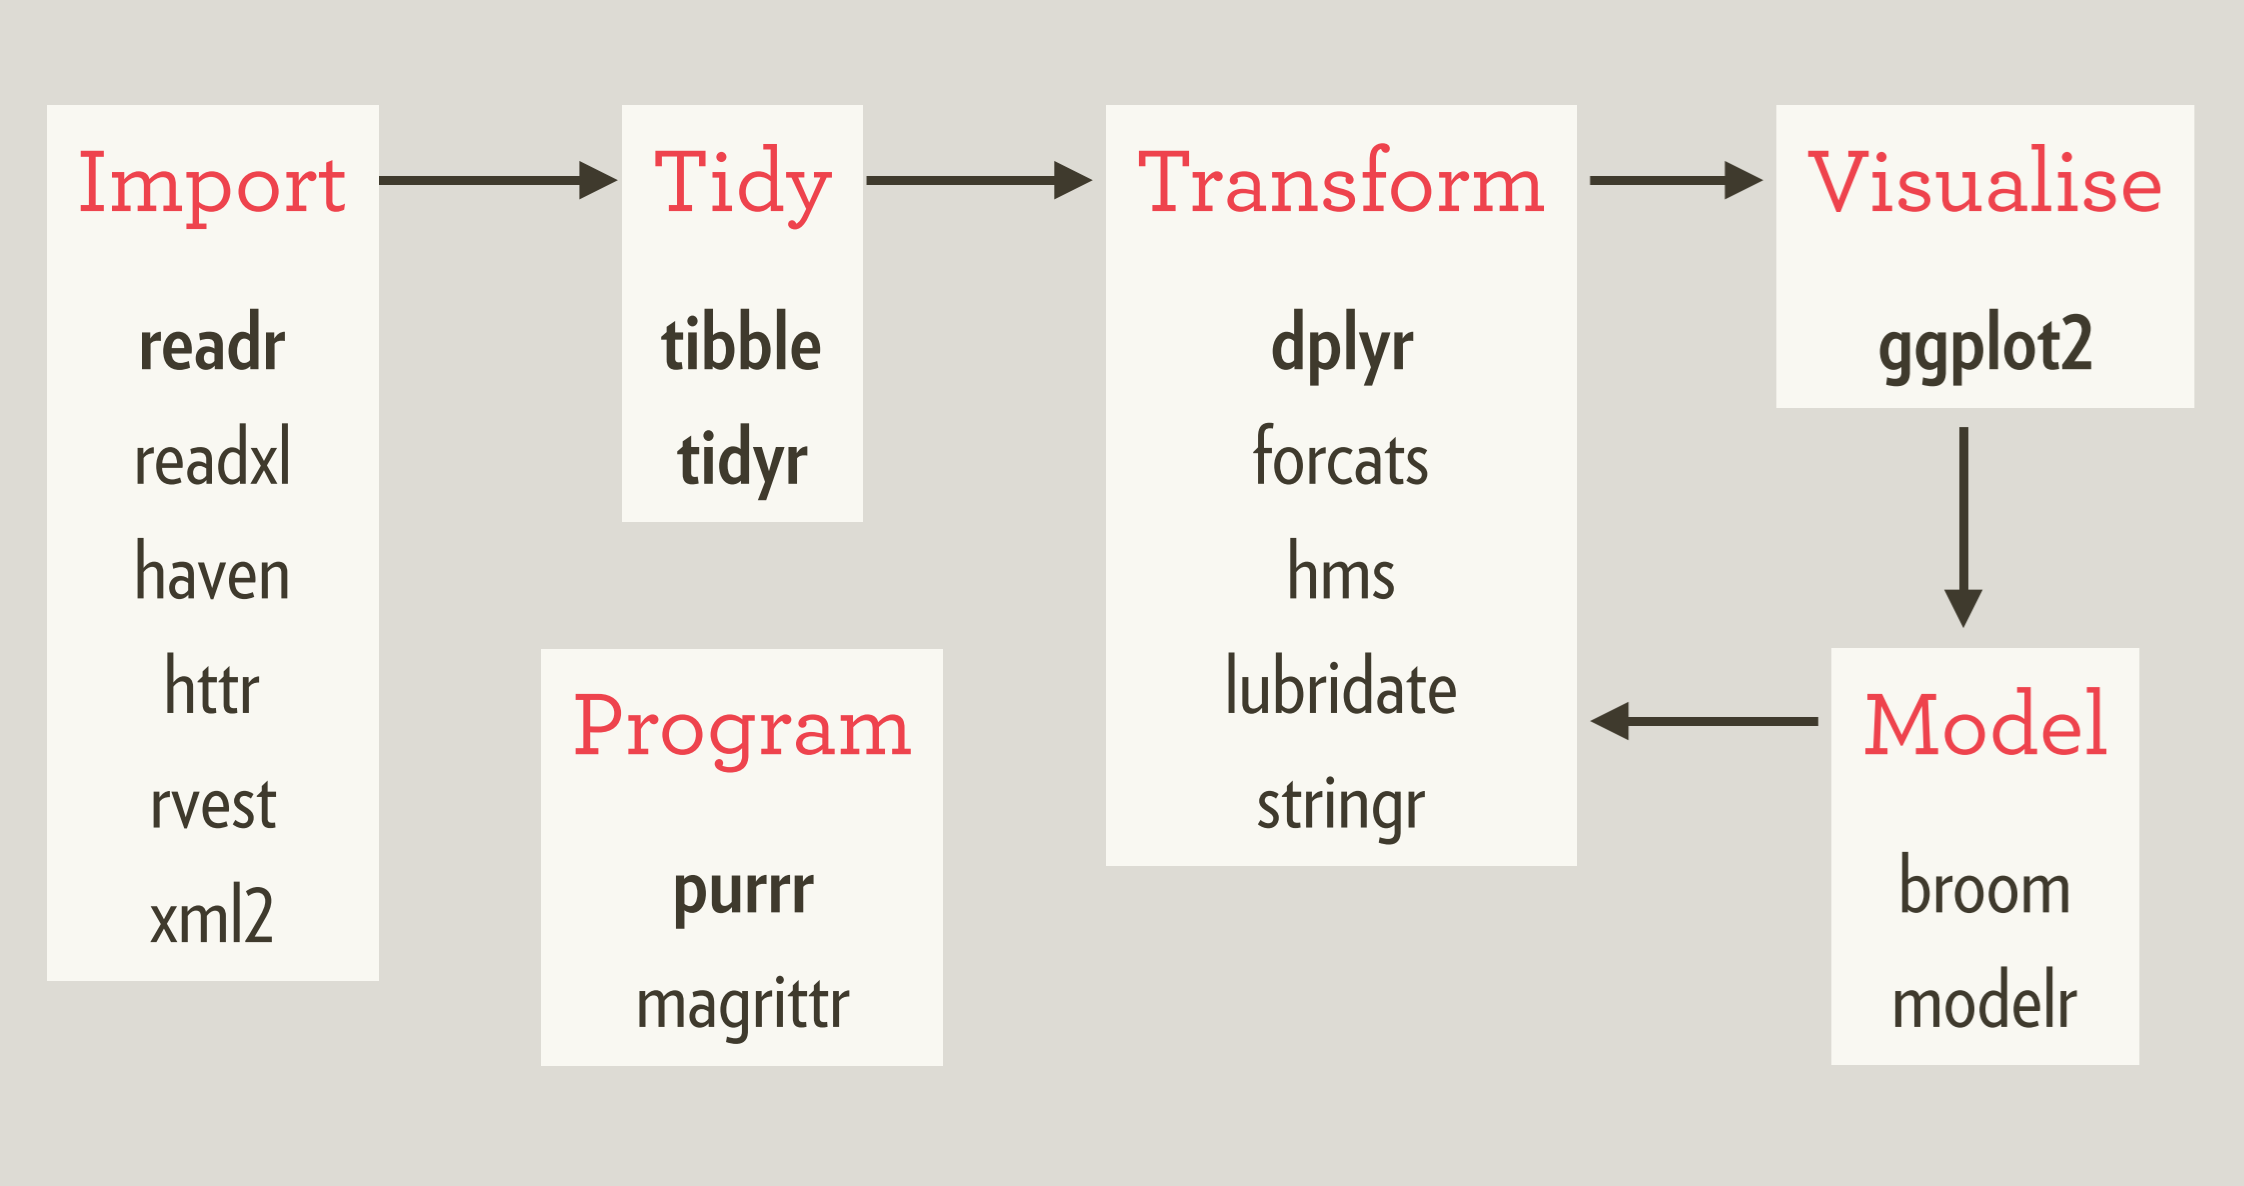
\includegraphics{images/tidyverse-workflow.png}
\caption{tidyverse 工作流}
\end{figure}

\begin{enumerate}
\def\labelenumi{\arabic{enumi}.}
\setcounter{enumi}{2}
\item
  tidyverse 用户众多,容易寻求帮助。 编写 R
  代码过程中遇到具体问题,可以到
  \href{https://stackoverflow.com/questions/tagged/r}{stack overflow}
  向全世界用户乃至开发者本人寻求帮助。
\item
  以 tidyverse 中某个包为依赖环境的拓展包不在少数,部分亦十分优秀(如
  dtplyr, dbplyr),学海无涯\ldots\ldots{}\footnote{dbplyr 可以实现与
    dplyr 语句结果等价的 SQL 数据库操作, 利用 dtplyr 可以实现间接调用
    data.table 包提高数据处理速度。}
\end{enumerate}

\hypertarget{ux672cux4e66ux4e0dux53cbux5584ux4e4bux5904}{%
\paragraph{本书不友善之处}\label{ux672cux4e66ux4e0dux53cbux5584ux4e4bux5904}}

\begin{enumerate}
\def\labelenumi{\arabic{enumi}.}
\item
  R
  语言本身语法内容较少,且在书中分布零散(例如对数据类型说明被排在第二十章)。
  这将致使读者难以对 \(R\) 语言有具体入微的理解与掌握。
  因此当我们开始处理本地个人项目时,比较容易陷入茫然无措的境地。
\item
  大概率成为 ``净土宗''
  的狂热信徒,表现为密集(强迫症)使用管道符。\footnote{由于在由管道符构建的局部环境中,我们以变量的形式索引数据(\href{https://cran.r-project.org/web/packages/dplyr/vignettes/programming.html}{dplyr
    verbs use tidy evaluation}),而在 R base
    原生环境中,当按变量名称索引数据时,我们只能使用变量的相应字符),这种设计固然在一定程度上为我们带来了书写代码的便捷,但与全局环境中命令语法的不统一,会使新手混淆索引数据的底层逻辑(何时变量名,何时必须使用字符)尤其是在管道符环境下调用本地编写的函数,稍有不慎,全局变量参数被按照字符进行传参,bug
    便如影随形\ldots\ldots{}}
\item
  tidyverse ``黑魔法''较多,写时优雅,但排除 bug 费时费力。 此外,近两年
  tidyverse 版本更新较快(以 Hadley 为首的开发团队庞大)。
  粗听起来这似乎是优点,但当你追逐潮流地更新包版本,重新跑之前写好的脚本,
  遇到奇怪的 bug 时,oh my god!
\end{enumerate}

\hypertarget{b.-the-art-of-r-programming-a-tour-of-statistical-software-design-by-norman-matloff---no-starch-press}{%
\subsubsection{\texorpdfstring{B. \emph{The Art of R Programming: A Tour
of Statistical Software Design} by Norman Matloff - No Starch
Press}{B. The Art of R Programming: A Tour of Statistical Software Design by Norman Matloff - No Starch Press}}\label{b.-the-art-of-r-programming-a-tour-of-statistical-software-design-by-norman-matloff---no-starch-press}}

本书面向的是对 R 有了一定的了解,想深入理解 R 的语法特性与数据对象,
以及提高 R 编程水平的入门读者。
尤其是适合拥有其它统计编程语言使用经验的学习者。

面对五花八门的数值,选择合适的数据类型(type)以及存储形态,
能极大地简化后续统计计算环节的语句。 作者在书中花费五章(共 110
页)详细叙述了 R 的数据结构 (\texttt{vector}, \texttt{array},
\texttt{list}, \texttt{data.frame}, \texttt{factor}),
这能为读者打下坚实的数据对象基础(尤其要牢牢掌握 vector, list,
data.frame)。 建议认真阅读本书\textbf{第二至第七章}内容。

\begin{figure}
\centering
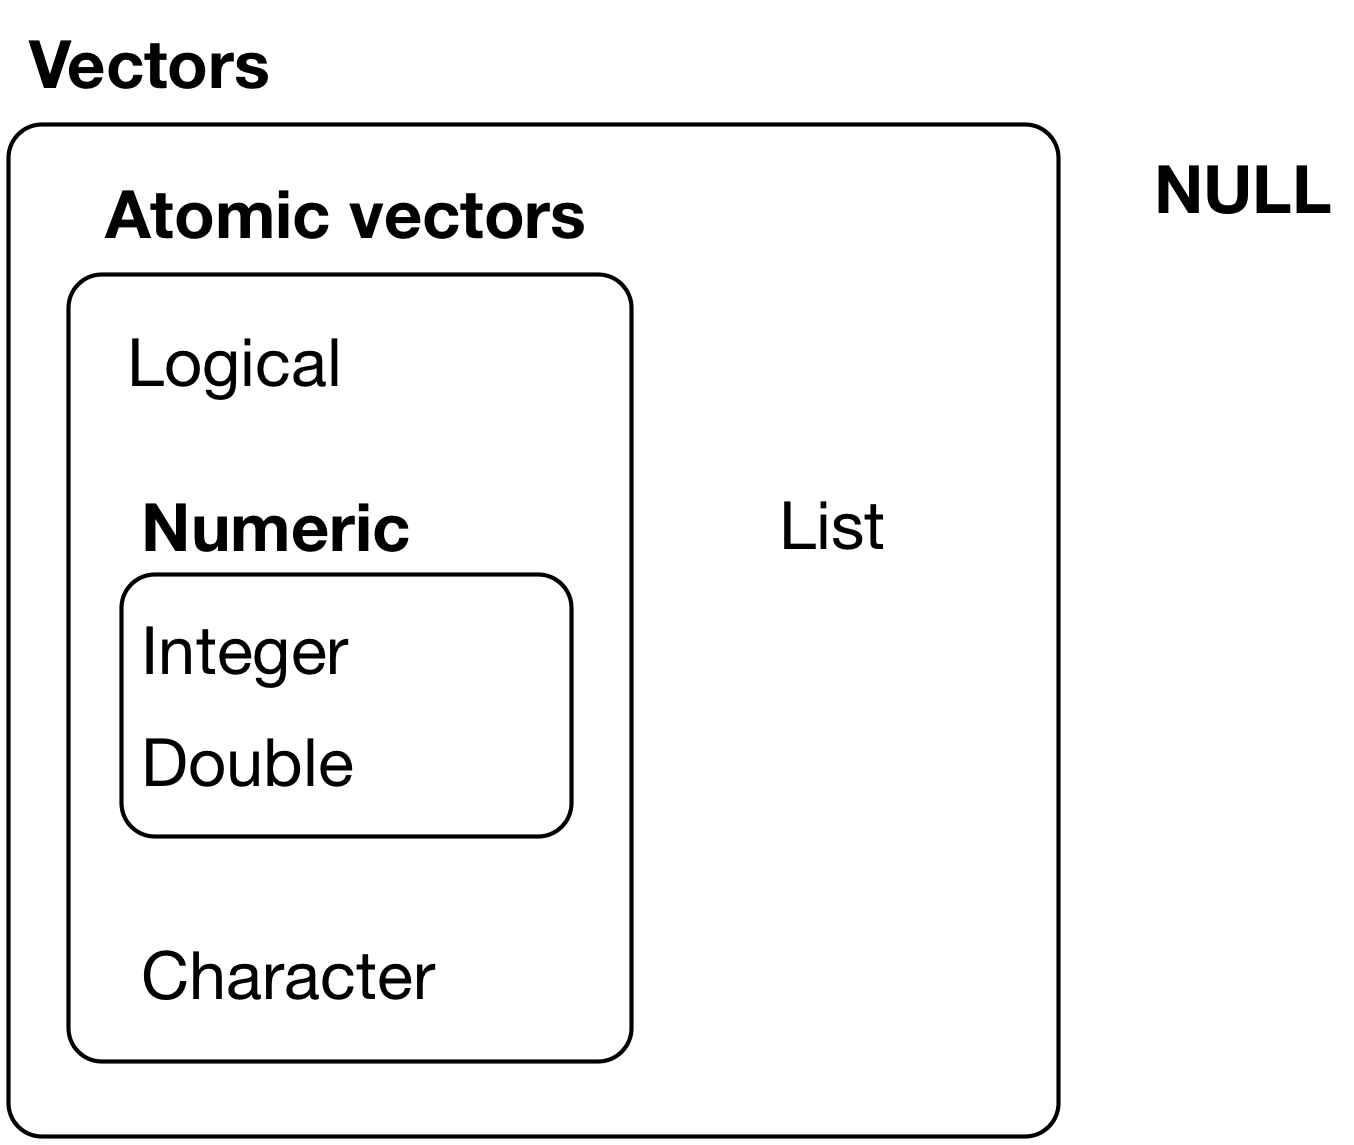
\includegraphics{images/data-structures.png}
\caption{R 数据结构}
\end{figure}

本书的令一大优点是同一个例子,作者会以渐进优化的逻辑实现两到三次(语句更简洁高效与通用)。
部分章节还附有一个综合性的例子,仔细琢磨这些例子能较好地提高我们应用 R
语言的水平,写出高质量的 R 代码。

\hypertarget{ux901aux8fc7ux9605ux8bfbux672cux4e66ux4f60ux5c06ux5b66ux5230}{%
\paragraph{通过阅读本书你将学到:}\label{ux901aux8fc7ux9605ux8bfbux672cux4e66ux4f60ux5c06ux5b66ux5230}}

\begin{enumerate}
\def\labelenumi{\arabic{enumi}.}
\item
  R 语言的底层逻辑,常用数据类型以及存储结构。
\item
  习惯于编写自己的函数,开启函数式编程之旅。\footnote{除了 if / for
    等基本程序循环控制流, \texttt{R\ base} 环境中的 \texttt{apply}
    族函数(我自己最常用的是 \texttt{lapply} 与 \texttt{sapply}),
    \texttt{purrr} 包中的 \texttt{map} 族函数(我自己最常用的是
    \texttt{map} 与 \texttt{map2},\texttt{map\_dbl} 与
    \texttt{map\_dfr})亦十分有必要掌握。 值得强调的是,\texttt{purrr}
    中的 \texttt{map} 族函数的威力在于与 list-colum
    式数据储存结构的结合使用。 此外,与 R base 的 \texttt{apply}
    族函数相比,\texttt{map} 族函数语法更加协调统一,易于记忆。
    若实在记不清,可在 \texttt{help()} 之外,配合\texttt{args()}
    直接查看函数参数设定情况(形参与实参,参数位置顺序等)。}
\item
  R 语句优化逻辑与思维。
\end{enumerate}

\hypertarget{c.-r-programming-for-data-science-by-roger-d.-peng---leanpub}{%
\subsubsection{\texorpdfstring{C.
\href{https://bookdown.org/rdpeng/rprogdatascience/}{R Programming for
Data Science} by Roger D. Peng -
Leanpub}{C. R Programming for Data Science by Roger D. Peng - Leanpub}}\label{c.-r-programming-for-data-science-by-roger-d.-peng---leanpub}}

学完上面两本稍偏技术层面的书,读者应该就能处理百分之九十以上的数据项目了。
接下来,学习 Peng 的这本 \emph{R Programming for Data Science}
一定程度上能为读者揭开 R 语言的面纱(以一种大巧若拙的高度应用 R)。

该书特点是,短则两三行,长则五六行,Peng
即能叙述清一个重要函数或某类操作的概念及用法。
且语言极其简洁精炼,每节内容很少超过一页纸。 Peng 为我们高屋建瓴地概述了
R 中常用数据操作的逻辑,并辅以简单的示例
(喜欢通过观看视频学习的同学(有外网环境),可直接经由每章开头的视频链接(Youtube)观看教学视频)。
阅读本书,能帮助我们从 \emph{The Art of R Programming}
的程序语言框架中跳出来,复以处理数据的视角审视 R。

通过学习本书,你将掌握:

\begin{enumerate}
\def\labelenumi{\arabic{enumi}.}
\item
  R 中基础函数(R base)的灵活使用。
\item
  码其然,知其所以然。如 R 为什么会有内存瓶颈(Scoping Rules of R)?
\item
  了解如何有效地优化某段 R 代码(从其实际占用 CPU 时间出发)以及 Debug
  的思路。
\item
  代码也要排版(8 个 space 为一个 Tab,每行内容不超过 80 个字符)!
\end{enumerate}

\hypertarget{d.-advanced-r-by-hadley-wickham---chapman-halls-r-series}{%
\subsubsection{\texorpdfstring{D.
\href{https://adv-r.hadley.nz/}{Advanced R} by Hadley Wickham - Chapman
\& Hall's R
Series}{D. Advanced R by Hadley Wickham - Chapman \& Hall's R Series}}\label{d.-advanced-r-by-hadley-wickham---chapman-halls-r-series}}

本书是第一本书 \emph{The R for data science} 的进阶版,
更多地站在开发者的角度讲解 R 的语法设计。 书中四分之三的内容由
programming 组成, 甚至包含 R \& C++ 内容。 对于只是拿 R
做统计计算的应用者而言,学习收益与时间成本不太划算。 更推荐熟练掌握
RStudio 公司制作的 cheat sheet.\footnote{cheat sheet 是以包为单位
  总结了(辅以可视化)包内部主体函数简单用法的一页 PDF。 一份好的 cheat
  sheet 能极大地帮助我们理解函数的用法(操作与目的),解放我们的记忆力。
  我们可根据自己的需求到 RStudio
  \href{https://rstudio.com/resources/cheatsheets/}{官方页面} 或该项目的
  \href{https://github.com/rstudio/cheatsheets}{Github 仓库}下载。
  一般来说,带有 cheat sheet 的包不会是差包。}

本书是本文所荐的四本技术书中我唯一没有读过的一本。
依然将其摆在这里,是我考虑到可能会有学弟妹已有一定的计算机科学基础,想无缝衔接到
R。 如是,则可直接上手 Hadley 大佬的这本 \emph{Advanced R}.

\hypertarget{e-ux5e72ux8d27ux89c6ux9891youtube}{%
\subsubsection{E
干货视频(Youtube)}\label{e-ux5e72ux8d27ux89c6ux9891youtube}}

\href{https://www.youtube.com/watch?v=_V8eKsto3Ug\&t=6s}{R Programming
Tutorial - Learn the Basics of Statistical Computing}

\href{https://www.youtube.com/watch?v=rz3_FDVt9eg\&t=3221s}{Hadley
Wickham: Managing many models with R}

\href{https://www.youtube.com/watch?v=49fADBfcDD4\&t=3498s}{Intro to
Data Visualization with R \& ggplot2}

\href{https://www.youtube.com/watch?v=7oyiPBjLAWY}{Code smells and
feels}

\href{https://www.youtube.com/watch?v=kuSQgswZdr8}{RStudio Tips and
Tricks}

\begin{center}\rule{0.5\linewidth}{0.5pt}\end{center}

\hypertarget{ux8ba1ux91cfux7ecfux6d4e-r}{%
\subsection{计量经济 \& R}\label{ux8ba1ux91cfux7ecfux6d4e-r}}

\begin{quote}
I've written thousands of lines of R, but never actually used it for
statistical analysis as opposed to using it as a functional programming
language.\\
--- Tom Lawton
\end{quote}

本人计量经济的水平十分有限,等同于大一新生(完全没学),
因此本节内容粗浅异常,读者可自寻通过别的渠道规划学习方案。

\hypertarget{a.-using-r-for-introductory-econometrics-by-florian-heiss---independently-published}{%
\subsubsection{\texorpdfstring{A. \href{http://www.urfie.net/}{Using R
for Introductory Econometrics} by Florian Heiss - Independently
published}{A. Using R for Introductory Econometrics by Florian Heiss - Independently published}}\label{a.-using-r-for-introductory-econometrics-by-florian-heiss---independently-published}}

我真正阅读过的应用 R 分析经济问题的只有这本 \emph{Using R for
Introductory Econometrics}. 在本书中,Florian Heiss 用 R 重现了
\emph{Introductory Econometrics: A Modern Approach} (by Jeffrey M.
Wooldridge) 书中所有例子的计量结果。
通过阅读本书,我们可以很快地明白如何通过调包调函数得到我们想要的计量结果。
本书缺点亦位于此: 规范的示例数据我们可以从 \texttt{woodlridge} 包 (by
Justin M. Shea and Kennth H. Brown) 中直接获取,
跑回归则直接一个函数命令结束。当我们处理自己的数据项目时,哪有这么爽歪歪的``老板''的待遇!
因此本书搭配 \emph{Introductory Econometrics}
可供高年级本科生学习,不太适合研究生。

值得强调的是,本书内容无缝衔接 Wooldridge 的计量教材 \emph{Introductory
Econometrics}, 能帮助我们更深入地理解 \emph{Introductory Econometrics}
书中的经典例子,而不是跑旁的乱七八糟的回归。

\hypertarget{b.-applied-econometrics-with-r-by-christian-kleiber-achim-zeileis---springer}{%
\subsubsection{\texorpdfstring{B.
\href{https://eeecon.uibk.ac.at/~zeileis/teaching/AER/}{Applied
Econometrics with R} by Christian Kleiber, Achim Zeileis -
Springer}{B. Applied Econometrics with R by Christian Kleiber, Achim Zeileis - Springer}}\label{b.-applied-econometrics-with-r-by-christian-kleiber-achim-zeileis---springer}}

触之所及,另一本 \emph{Applied Econometrics with R} 十分值得推荐。
此书作者不仅花费大段文字提点我们在应用某包函数跑某类计量模型时的逻辑与注意事项(难得的经验),
还给出了核心统计量的数学表达式(矩阵形式)。\footnote{写到这里,很后悔为什么我没有在接触到这本书的当时就啃它(文档下载时间显示我是
  2018 年 12 月 12 日知晓本书存在的),
  希望以学术为志的学弟妹引以为戒,不要花太多时间在学习数据处理技术上,核心的应该是掌握回归模型的计算推导,以及模型背后的经济学阐释。}
此书还有一个高大上的简称 \emph{AER},本书的相应包 \texttt{AER} 亦被
\emph{CRAN} 收录。

\hypertarget{c.-econometrics-in-r-by-grant-v.-farnsworth}{%
\subsubsection{\texorpdfstring{C.
\href{https://cran.r-project.org/doc/contrib/Farnsworth-EconometricsInR.pdf}{Econometrics
in R} by Grant V.
Farnsworth}{C. Econometrics in R by Grant V. Farnsworth}}\label{c.-econometrics-in-r-by-grant-v.-farnsworth}}

此处我还想题一题另一份只有五十页的 \emph{Econometrics in R} . 该文档中
Cross Sectional Regression, Special Regression Time Series Regression
三节内容只占十页,半天即可读完。
读者可凭此快速了解跑某类计量经济模型有哪些包可供选择(缺点是本文写于
2008 年年底,比较旧了)。

\hypertarget{d.-cran---task-views}{%
\subsubsection{\texorpdfstring{D.
\href{https://mirrors.tuna.tsinghua.edu.cn/CRAN/web/views/}{CRAN - Task
Views}}{D. CRAN - Task Views}}\label{d.-cran---task-views}}

\begin{quote}
CRAN task views aim to provide some guidance which packages on CRAN are
relevant for tasks related to a certain topic.
\end{quote}

我们可到 CRAN 的 Tasks Views
页面扫览有哪些代表性的包可被应用于本学科统计计算任务。 CRAN 上的 tasks
大致是基于统计学科的子领域和学科应用范围划分的
(相当于可供学院开设一至两个学期的专业选修课)。 与经济相关的有
\href{https://mirrors.tuna.tsinghua.edu.cn/CRAN/web/views/Econometrics.html}{Econometrics},
\href{https://mirrors.tuna.tsinghua.edu.cn/CRAN/web/views/Finance.html}{Finance},
\href{https://mirrors.tuna.tsinghua.edu.cn/CRAN/web/views/TimeSeries.html}{TimeSeries},
\href{https://mirrors.tuna.tsinghua.edu.cn/CRAN/web/views/Robust.html}{Robust}.
各 task 下的内容按模型方法划分,
对我们会遇到的统计计算任务,两三句话告知我们有哪些相关的包可供调用。

\begin{center}\rule{0.5\linewidth}{0.5pt}\end{center}

\hypertarget{ux9047ux5230ux95eeux9898ux5982ux4f55ux89e3ux51b3}{%
\subsubsection{遇到问题如何解决}\label{ux9047ux5230ux95eeux9898ux5982ux4f55ux89e3ux51b3}}

\begin{enumerate}
\def\labelenumi{\arabic{enumi}.}
\item
  通过 \(R\) 内置的帮助系统(\texttt{?},
  \texttt{help()})以及参数查询函数 \texttt{args()}
  深入了解某一函数用法;
\item
  善用 \href{https://www.google.com/}{搜索引擎} 与程序语言问答网站
  \href{https://stackoverflow.com/questions/tagged/r}{stack overflow};
\end{enumerate}

我们遇到的大多数问题网友都曾遇到过,因此网络上基本都有答案,顶多需要我们对多个解决方案进行比较与重组。
此外,阅读网友的解决方案或示例代码,不光能解决我们遇到的某类问题,也能加深我们对语法的理解;

\begin{enumerate}
\def\labelenumi{\arabic{enumi}.}
\setcounter{enumi}{2}
\tightlist
\item
  查阅 R 官方给出的常见
  \href{https://mirrors.tuna.tsinghua.edu.cn/CRAN/faqs.html}{FAQs} 与
  \href{https://mirrors.tuna.tsinghua.edu.cn/CRAN/manuals.html}{The R
  Manuals}
\end{enumerate}

需要注意的是,R Manuals
更多面向的是开发者与服务器平台用户(在教读者如何安装以及管理 R
的子文档中,Installing R under Unix-alikes 排在了 Installing R under
Windows 与 Installing R under macOS 前面)。
站在应用的层面,只建议有针对性地查阅 An Introduction to R, R Data
Import/Export 两份主文档(利用浏览器内置的文本搜索功能,在 HTML
页面检索答案)。 学习到这里,你大概已经是两个 \(\sigma\) 的 R 中毒者了!

\hypertarget{ux5305ux7684ux98dfux7528ux65b9ux6cd5}{%
\subsubsection{包的食用方法}\label{ux5305ux7684ux98dfux7528ux65b9ux6cd5}}

R
中的包由三部分内容组成:函数(包的主体内容),帮助文档(用法说明),以及示例数据。
如何系统地了解包内附有哪些函数,以及这些函数的具体用法?\footnote{\href{https://www.r-bloggers.com/essential-list-of-useful-r-packages-for-data-scientists/}{Essential
  list of useful R packages for data scientists},
  这是一份网友站在统计学者和数据科学的角度给的一份 R 包清单。 Many
  useful functions are available in many different R packages, many of
  the same functionalities also in different packages, so it all boils
  down to user preferences and work, that one decides to use particular
  package.}

最直接高效的方式就是到该包主页看有无语法说明, 被 CRAN
收录的包的网络地址格式为
\url{https://cran.r-project.org/package=dplyr}。 其中\texttt{dplyr}
是我输入的示例包名,当我们查询欲浏览某包主页,我们只需将其替换为我们相应包名。
如我们现在想看 \texttt{ggplot2} 主页,我们在浏览器的网址栏输入
\url{https://cran.r-project.org/package=ggplot2}, 回车即可开始冲浪。
我们主要看页面中哪些内容呢?

\begin{itemize}
\item
  In views

  通过页面中的 In views 条目,我们可以知晓该包被哪些 tasks
  索引(其定位)。
\item
  Materials - README

  README 一般都包含有 Overview, Installation, Usage 三部分内容。
  友好的开发者会在文内对包的核心函数做简略介绍,对大多数用户而言,熟练掌握这些就够了。
\item
  Vignettes

  对包内主要函数及语法更详细的说明,经常附带些``黑魔法''。
  建议耐心阅读。
\item
  Reference manual

  Reference manual 是作者遵照 R 社区包开发标准,
  对此包内部所有函数的完整介绍(包括描述介绍、函数参数、示例代码等)。
  文档常长达百页(为兼顾阅读舒适性,排版较为稀疏)。\footnote{此处为 pdf
    文档,pdf 格式的帮助手册的优势是可集中学习,不用在 HTML
    页面来回跳转。 其实,该份 manual 手册已被 R 内置了超链接索引。
    还是以包 \texttt{dplyr} 为例,我们只要在 R 终端(console)输入
    \texttt{help(package\ =\ "dplyr")} 并回车,
    就能在默认浏览器打开该包的 Reference manual 手册(HTML)。
    若是在集成编辑器 RStudio 中敲相应命令,手册将直接显示在 Help
    窗口(不能白白占用四五百 MB 的内存啊)。
    当然,我们也记不住那么多的函数(哪些是实参,哪些是形参)。
    我们更多的还是以查询工具书的方式浏览它。}
\end{itemize}

\hypertarget{ux4ee5-r-ux5305ux4e3aux5356ux70b9ux7684ux4e24ux672cux671fux520a}{%
\paragraph{以 R
包为卖点的两本期刊}\label{ux4ee5-r-ux5305ux4e3aux5356ux70b9ux7684ux4e24ux672cux671fux520a}}

\begin{itemize}
\tightlist
\item
  \href{https://journal.r-project.org/}{The R Journal}
\end{itemize}

The R Journal 是 R 官方编辑的期刊,拥有 ISSN 编号,一年两期。
每篇论文以一个新包为叙述主体(作者为实现某类统计计算方法所开发),
论文可供随意下载,并附有示例 R 代码。 文内的包大多遵循 Creative Commons
Attribution 4.0 International license,
即只要非商业用途,署上作者名便可随意使用。

\begin{itemize}
\tightlist
\item
  \href{https://www.jstatsoft.org/index}{Journal of Statistical
  Software}
\end{itemize}

JSS 期刊是我在搜索引擎检索某个 R 语言问题时发现的, 同 The R Journal
一样,志在曝光新包,论文与示例代码可通过杂志官网超链接直接获取。
并附有包的源码(避免未被 CRAN 收录的可能)。 The R Journal 与 JSS
双管齐下,保准你站在 R 浪头之巅。

\hypertarget{ux5bf9-tidyverse-ux7cfbux5217ux5305ux7684ux8865ux5145ux8bf4ux660e}{%
\subsubsection{对 tidyverse
系列包的补充说明}\label{ux5bf9-tidyverse-ux7cfbux5217ux5305ux7684ux8865ux5145ux8bf4ux660e}}

\begin{itemize}
\item
  readr \& tidyr \& tibble

  readr 负责定制化读取数据, tidyr
  负责将我们的数据整理成列(column)为变量(特征),行(row)为观测对象(单个样本)的
  tabular data, tibble 增强了 R 中 data.frame
  数据在终端中的阅读性,统一了对 data.frame
  中数据做索引时返回值的数据属性。\footnote{一定程度上能避免产生自己难以意识到的数据结构层面的
    bug。 举例来说,从 data.frame 中单取出一列数据,返回值依然是
    data.frame 还是一维的向量,视索引函数而定,而不依赖于数据的维度。}
\end{itemize}

\begin{figure}
\centering
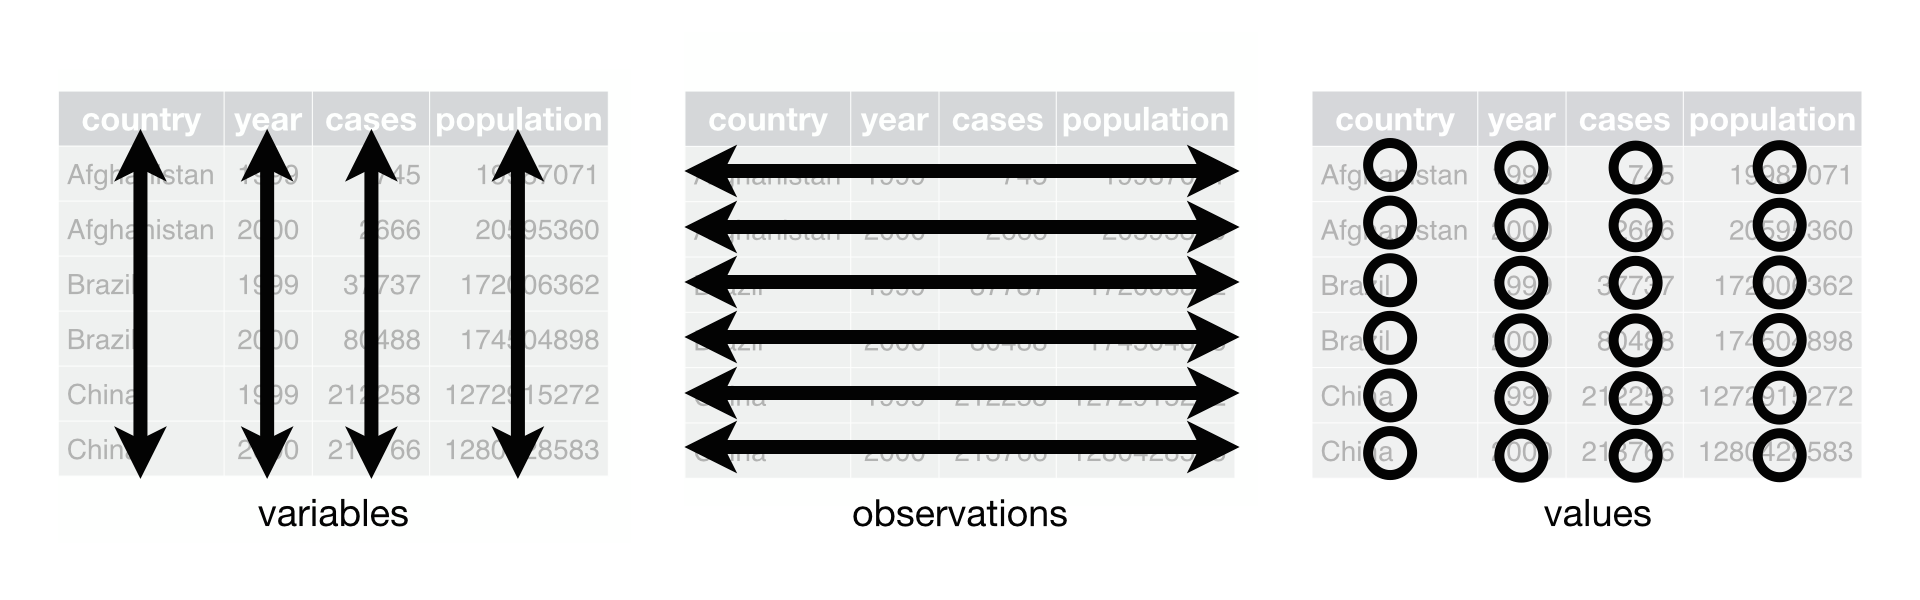
\includegraphics{images/tidy.png}
\caption{tabular data}
\end{figure}

\begin{itemize}
\item
  dplyr

  dplyr 是 tidyverse 的核心,应用主要有三个方面,\footnote{dplyr
    vs.~data.table. data.table 是 R 中另一个十分优秀的数据操作包。
    data.table
    会隐式地根据目标任务展开并行计算,优化内存占用量,计算速度表现十分出众。
    data.table 的逻辑与 tidyverse 的逻辑可以说是完全相反。 tidyverse
    强调语句的直观性,辅以大量各具特色的函数,企图让数据操作语句成为一套优雅的拳法;
    而 data.ble 语法就像是陈咬金的三板斧,虽然就一招三参量,但依凭复杂的
    R 基础语句(绝对的抽象),依然可实现复杂的数据操作。}

  \begin{enumerate}
  \def\labelenumi{\arabic{enumi}.}
  \item
    简洁且自动化程度高(如 select\_*
    族函数)地对行列做筛选;添加列变量,包括对 data.fram
    中已有变量做数据变化(取对数等),对多列变量做线性组合等。
  \item
    多对个 data.frame 做各式各样的合并操作(*\_join
    族函数,交、并、补)。
  \item
    \texttt{group\_by()} 函数 + \texttt{summarise()} 函数 +
    科学计算表达式或内置计算函数。熟练掌握此套招数,计算以及比较不同组别间的数据统计量变得非常简单,代码也十分简洁优雅!
  \end{enumerate}
\item
  purrr

  purrr 构建的 list-column workflow (column-wise programming)
  优雅非常!将分散的数据结果(以 list
  为基本数据单位)以列的形式集合到一张表之后,我们借助 \texttt{map}
  族函数在行(row)之间实现隐式循环操作,在列(column)之间存储阶段性编程结果。
\end{itemize}

\hypertarget{ux8865ux5145ux7f51ux7ad9-ux8bbaux575b}{%
\subsubsection{补充网站 \&
论坛}\label{ux8865ux5145ux7f51ux7ad9-ux8bbaux575b}}

\begin{itemize}
\tightlist
\item
  \url{https://bookdown.org/}
\end{itemize}

\href{https://yihui.org/}{谢益辉}谢大开发的一系列 \texttt{*down}
包为我们撰写各类文档文件提供了极大的助益,本站是 bookdown 的官网,
一系列基于 bookdown 攥写的书籍开源于此。 上文我推荐的书籍 \emph{R for
Data Science} 和 \emph{R Programming for Data Science} 皆在列表之中。
大家可根据自己的数据项目需求,选择某一主题的书进行强化阅读。\footnote{此处有必要提一嘴由谢大个人单枪匹马开发的
  \texttt{R\ markdown}。 \texttt{R\ markdown} 在 R 的基础之上,利用
  knitr 包让生成可重复性研究报告变得轻而易举, 并且借助 pandoc
  让我们可以随意选择文档输出格式(本文即是用 R markdown 写的)。
  站在对受众的影响和受众的范围来讲,R markdown 的产品杰出程度甚至要超过
  tidyverse。 感兴趣的请移步
  \href{https://robjhyndman.com/seminars/rmarkdown/}{How Rmarkdown
  changed my life}. 此外,谢大的\href{https://yihui.org/}{个人主页}上 -
  演讲和讲座 - 栏目亦是干货满满,塞满了其四处演讲的幻灯片!
  我研一上学期非常喜欢读谢大的博客(最早可追溯到 2005
  年年初),文字纯真而富有启迪。}

\begin{itemize}
\tightlist
\item
  \href{https://cosx.org/}{统计之都}
\end{itemize}

由谢大发起并创办的统计之都是国内最专业的统计知识交流社区。
主页的文章干货满满,三十几期的专访(统计学者为主)是我等菜鸡不竭的鸡汤来源。
其下论坛也有 \href{https://d.cosx.org/t/r}{R
子板},坛友之间纯交流技术和统计学问题。
无娱乐无政治无新闻,也不是乱七八糟的资源分享站,清净而能学到东西。

\begin{itemize}
\tightlist
\item
  \href{https://www.r-graph-gallery.com/index.html}{The R Graph Gallery}
\end{itemize}

一个展示如何利用 tidyverse 和 ggplot2
做数据可视化的网站,每张图片的下方便是相应的 R 代码。
该网站除却数据图形非常齐全,更难得的是附带的绘图代码写的非常规范,且基本做到了每行命令皆有注释说明,
十分适合对数据可视化有兴趣的同学浏览学习
(最好是读过一两本讲述数据可视化的书籍,有一定的数据科学常识和图形品味之后)。
这里推荐一本书 \href{https://serialmentor.com/dataviz/}{Fundamentals of
Data Visualization},

\begin{quote}
The book is meant as a guide to making visualizations that accurately
reflect the data, tell a story, and look professional. In my experience,
scientists frequently (though not always!) know how to visualize data
without being grossly misleading. However, they may not have a well
developed sense of visual aesthetics, and they may inadvertantly make
visual choices that detract from their desired message. Designers, on
the other hand, may prepare visualizations that look beautiful but play
fast and loose with the data. It is my goal to provide useful
information to both groups.\\
--- Claus O. Wilke
\end{quote}

\begin{itemize}
\tightlist
\item
  \url{https://www.r-bloggers.com/}
\end{itemize}

该网站的定位是: \emph{R news and tutorials contributed by hundreds of R
bloggers}. 一天博客的发布量在三到十条左右。
阅读这些博客可以极大拓展地我们的数据视野,避免我们自身陷入技术孤岛。

\begin{figure}
\centering
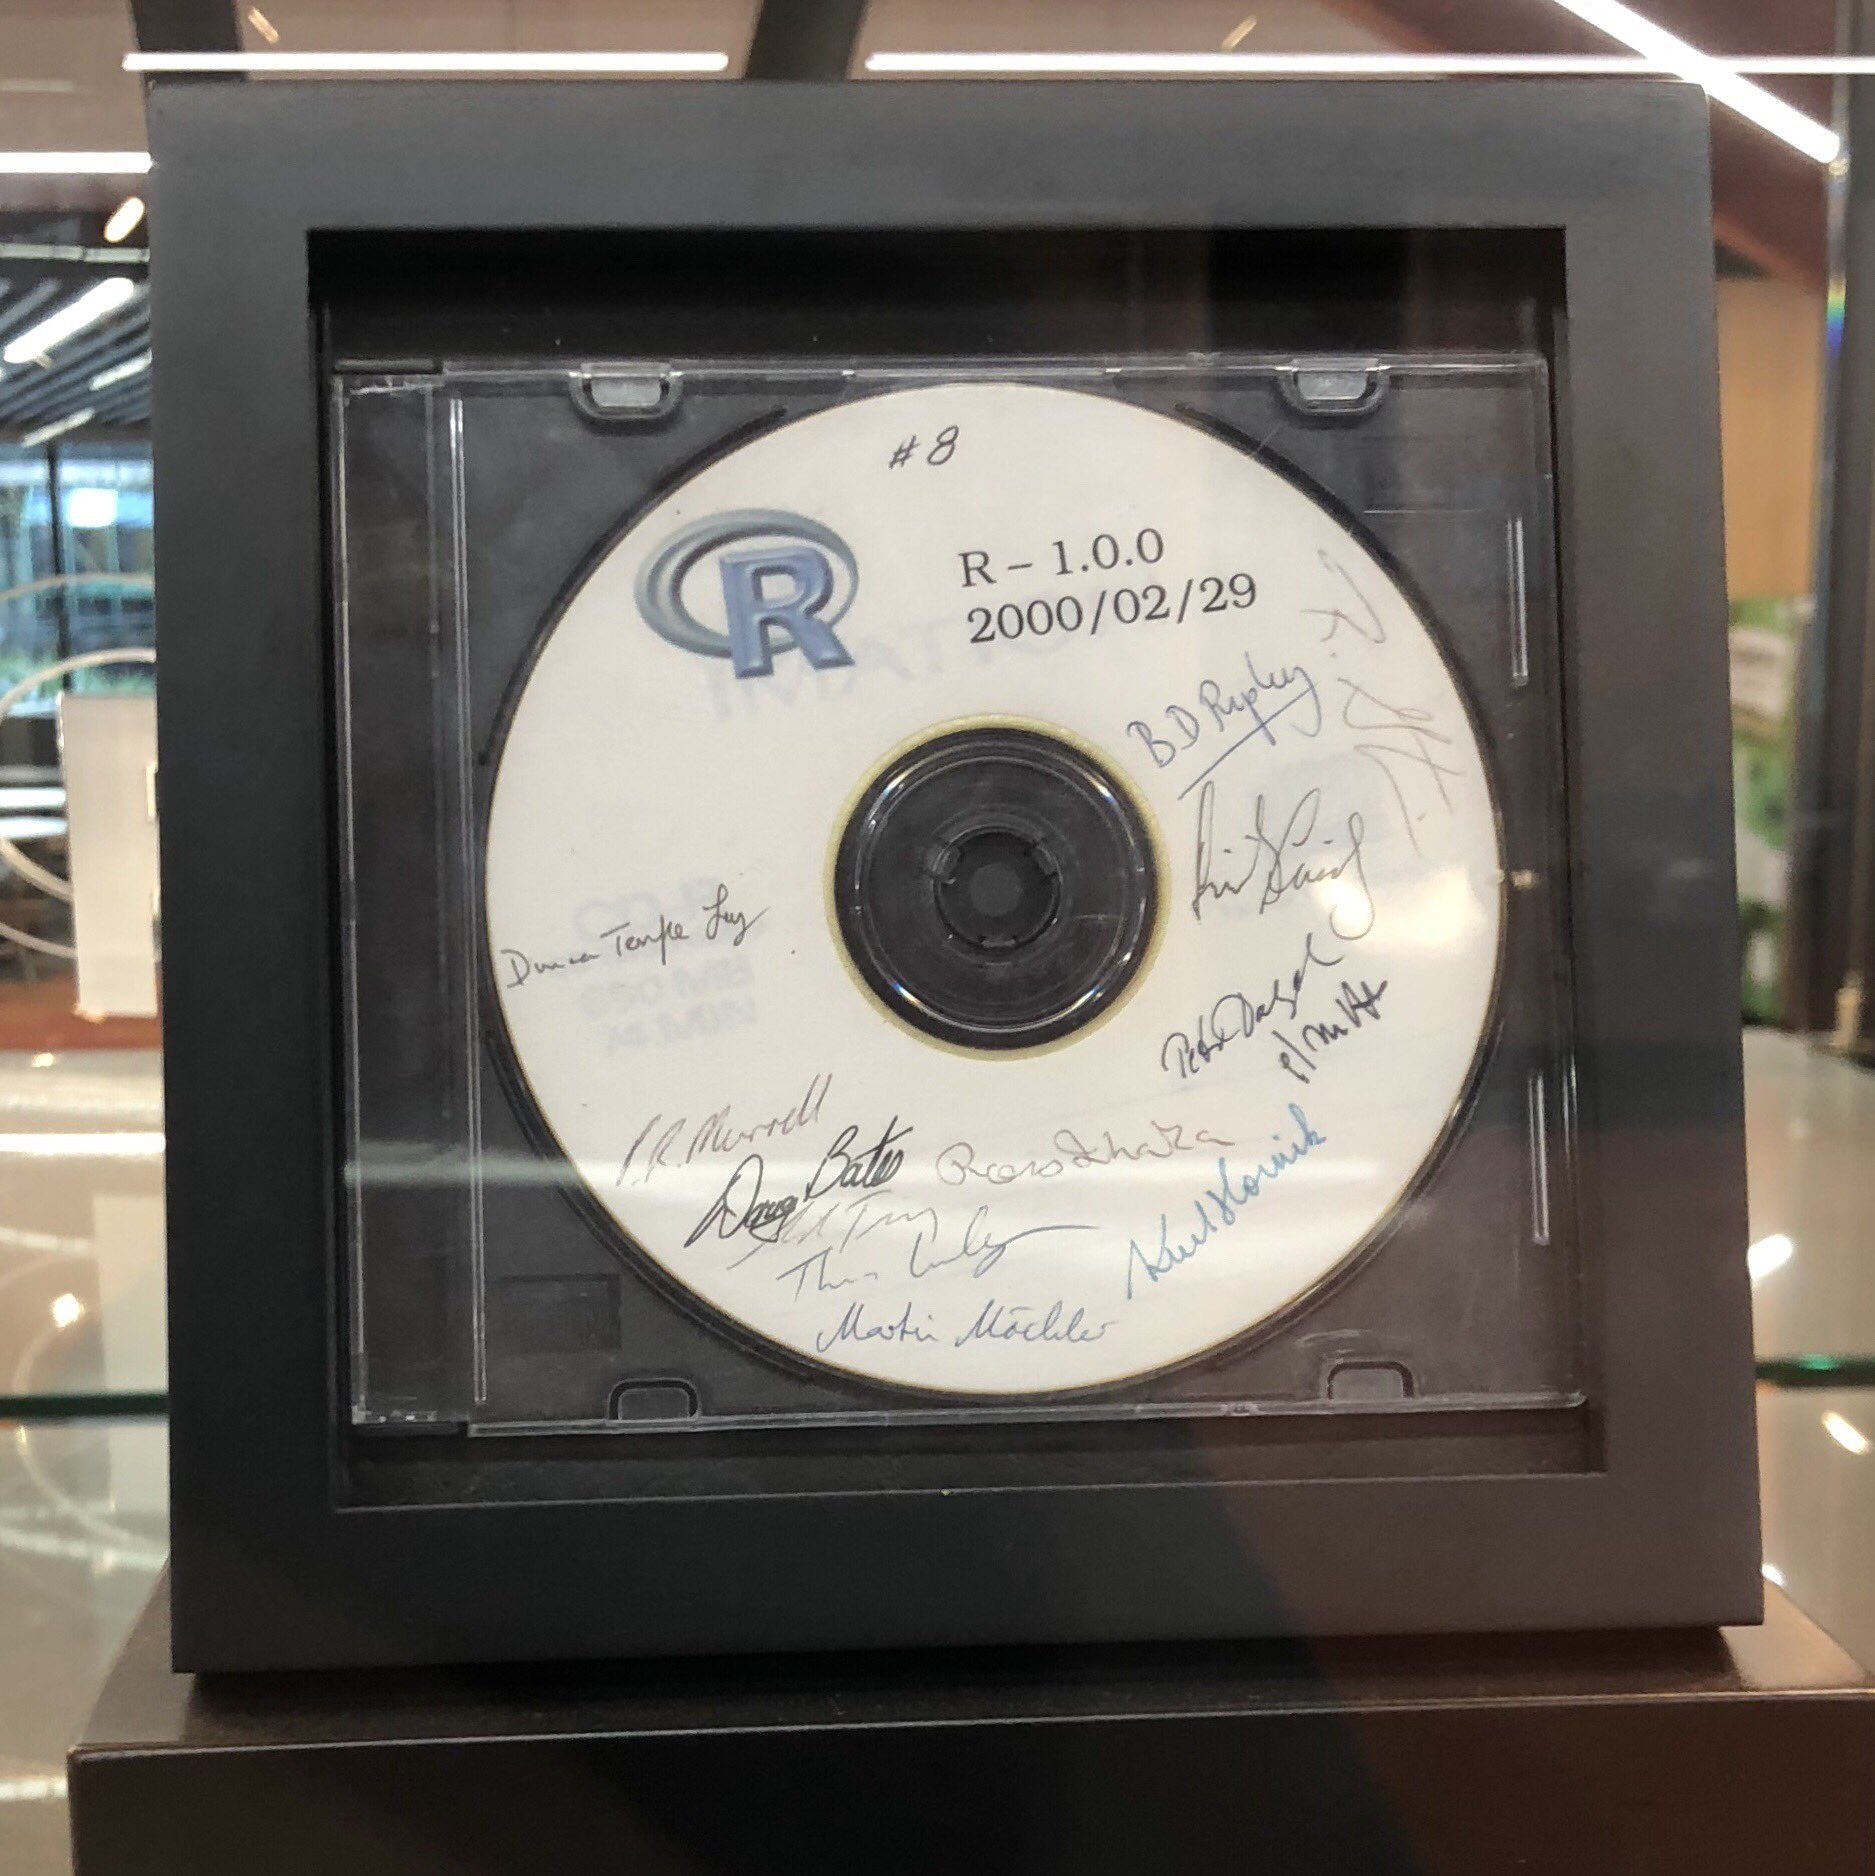
\includegraphics{images/A-CD-ROM-of-the-original-version-of-R-signed-by-the-R-Core-Team.jpg}
\caption{布满 R 核心开发团队成员签名的 R 1.0.0 版 CD}
\end{figure}

\end{document}
